
\documentclass[MAIN.tex]{subfiles} 
\begin{document} 
	\begin{frame}
		\frametitle{Probability Distributions}
	A probability distribution is a table or an equation that links each outcome (or range of outcomes) 
	of a statistical experiment with its probability of occurrence.\\
	\bigskip
	\textbf{Two Families}
	\begin{itemize}
	\item Discrete Distributions (i.e. Count Variables  - Integers )
	\item Continuous Distributions (i.e. Continuous Variables - Real Numbers )
	\end{itemize}
	
	\end{frame}
%================================================================================== %
\begin{frame}
	\frametitle{Discrete distributions}
\begin{itemize}
\item Benford Distribution
\item Bernouilli distribution
\item Binomial distribution
\item Hypergeometric distribution
\item Geometric distribution
\item Multinomial distribution
\item Negative binomial distribution
\item Poisson distribution
\item Zipf's law
\end{itemize}
\end{frame}

%================================================================================== %
\begin{frame}
\frametitle{Continuous distributions}
\begin{itemize}
\item Beta and Dirichlet distributions
\item Cauchy distribution
\item Chi Square distribution
\item Exponential distribution
\item Fisher-Snedecor distribution
\item Gamma distribution
\item Levy distribution
\item Log-normal distribution
\item Normal and related distributions
\item Pareto Distributions
\item Student's t distribution
\item Uniform distribution
\item Weibull distribution
\item Extreme values and related distribution
\item Distribution in circular statistics
\end{itemize}
\end{frame}
%================================================================================== %
\begin{frame}
	\begin{figure}
		\centering
		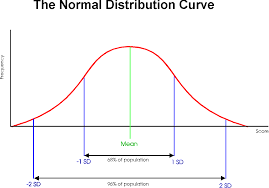
\includegraphics[width=0.9\linewidth]{images/bellcurve}
	\end{figure}

\end{frame}
%================================================================================== %
\begin{frame}
\frametitle{The Normal Distribution}
\textbf{Normal Probability Distribution}
\large
\begin{itemize}
\item Cornerstone of every undergraduate statistics module.
\item Basis of a substantial body of statistical theory
.\item Central Limit Theorem - basis of Statistical Inference (i.e. Hypothesis Tesing, Confidence Intervals).

\end{itemize}
\end{frame}
%================================================================================== %
\begin{frame}
\frametitle{Compendium of Probability Distributions}
\begin{figure}
\centering

\includegraphics[width=1.05\linewidth]{images/vosecompendium}
\end{figure}
\end{frame}
%================================================================================== %
\begin{frame}
	\frametitle{Compendium of Probability Distributions}
		\begin{figure}
\centering
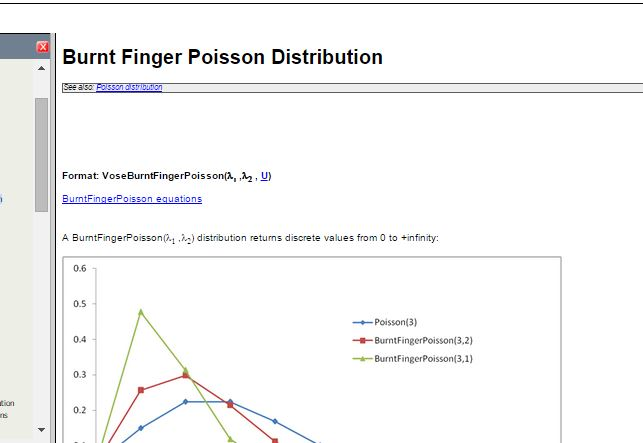
\includegraphics[width=0.9\linewidth]{images/burntfinger}

\end{figure}

\end{frame}
%================================================================================ %
\begin{frame}
	\frametitle{Compendium of Probability Distributions}
\textbf{Burnt Finger Poisson Disribution}
\begin{itemize}
\item This type of situation occurs when, for example, an individual has an expected rate of accidents $\lambda_1$, but if an accident occurs the individual will become more careful (his/her ``fingers got burned") so that for the rest of the modeled time a new, lower expected accident rate $\lambda_1$ applies.
\end{itemize}
\end{frame}
%================================================================================= %
\begin{frame}
	\frametitle{Main Functions for \texttt{R}}
\begin{description}
\item[\texttt{d}] - probability density function
\item[\texttt{p}] - cumulative distribution function
\item[\texttt{q}] - quantile function
\item[\texttt{r}] - random number generation function
\end{description}

\end{frame}

\begin{frame}
	\begin{figure}
\centering
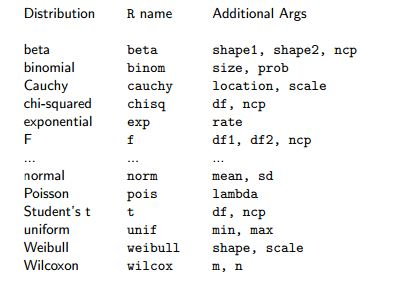
\includegraphics[width=0.9\linewidth]{images/stems}
\caption{}
\label{fig:stems}
\end{figure}

	
\end{frame}
%================================================================================= %
\begin{frame}
	\begin{figure}
\centering
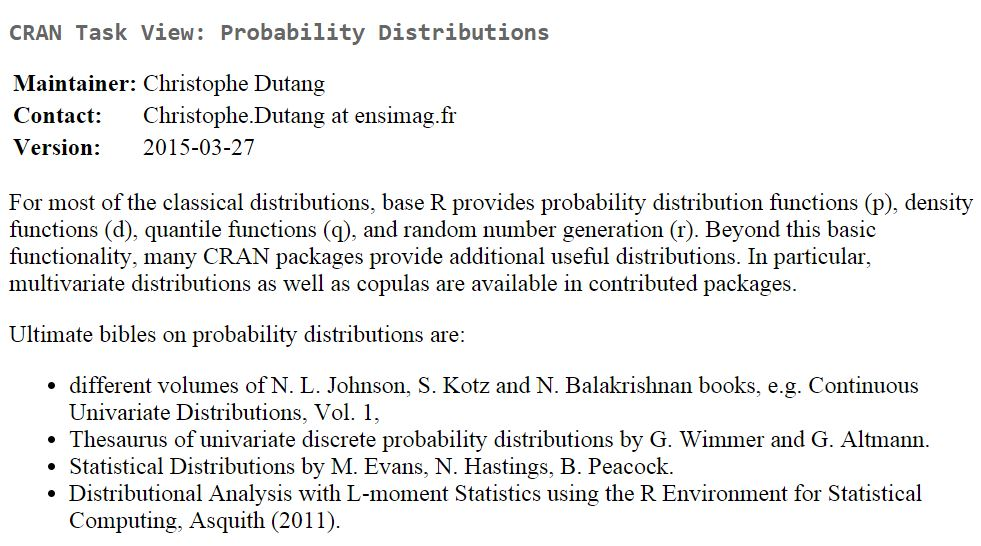
\includegraphics[width=1.05\linewidth]{images/CRANTaskview}

\end{figure}
\end{frame}
%================================================================================= %
\begin{frame}
	
\begin{figure}
\centering
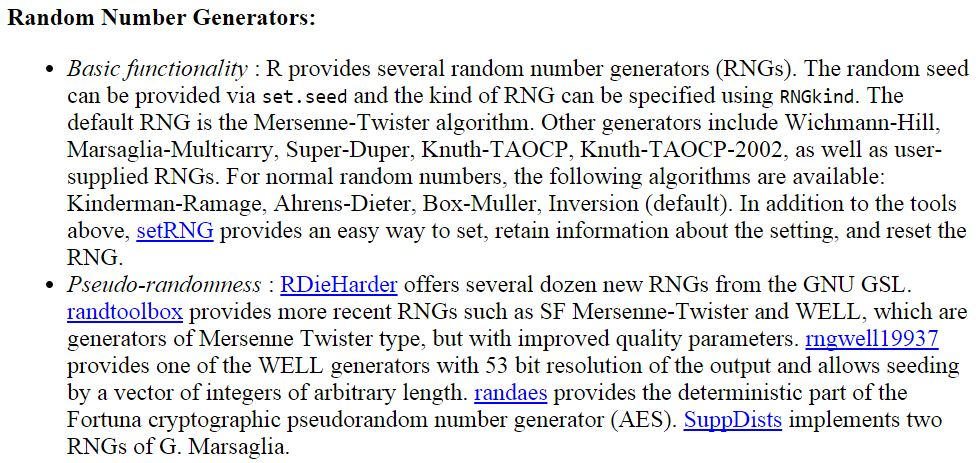
\includegraphics[width=0.7\linewidth]{images/CRANrng}
\caption{}
\label{fig:CRANrng}
\end{figure}

\end{frame}
%================================================================================= %
\begin{frame}
	\begin{figure}
\centering
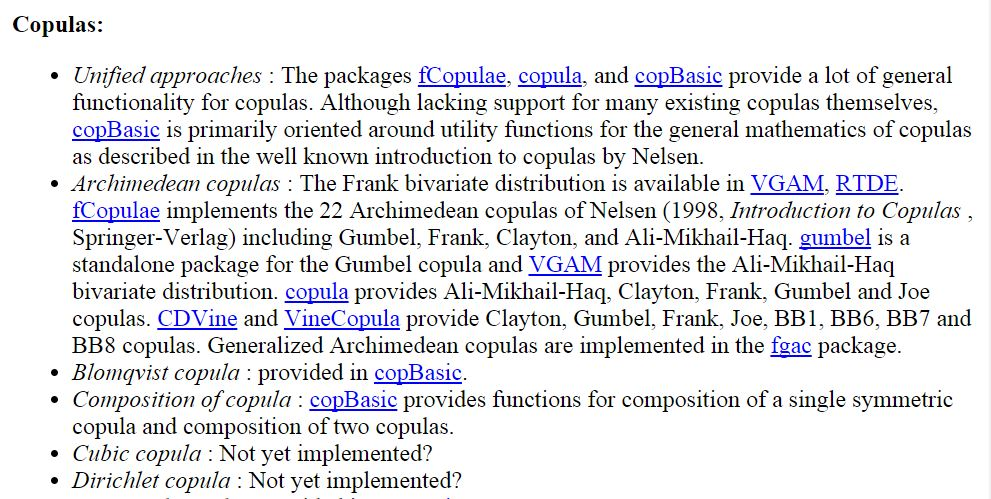
\includegraphics[width=0.7\linewidth]{images/CRANcopulas}
\caption{}
\label{fig:CRANcopulas}
\end{figure}

\end{frame}
%================================================================================= %
\end{document}
